\documentclass{article}


\usepackage[left=3cm,right=3cm,top=2cm,bottom=3cm]{geometry} % page settings
\usepackage{amsmath,amsfonts,amsthm,amssymb} % provides many mathematical environments & tools


\usepackage{tikz}
\usetikzlibrary{shapes,arrows,positioning}
\usetikzlibrary{mindmap,trees, backgrounds}
\usetikzlibrary{decorations.pathreplacing}


\tikzset{block/.style={rectangle, draw, text width=10em, text centered, rounded corners,
 minimum width=3.5cm}}
 \tikzset{blockL/.style={rectangle, draw, text width=14em, text centered, rounded corners,
 minimum width=3.5cm}}
\tikzset{block_color/.style={rectangle, draw, fill=BurntOrange!65, text width=10em, text centered, rounded corners,
 minimum width=3.5cm}}
 \tikzset{line/.style={draw, -latex}}
 
 \definecolor{green_m}{rgb}{0.0, 0.66, 0.47}
 
 
\usepackage{adjustbox}

\usepackage{bigints}
\usepackage{hyperref}
\newcommand{\lver}{\left|}
\newcommand{\rver}{\right|}
\newcommand{\bsy}[1]{\boldsymbol{#1}}

\usepackage{hyperref}
\hypersetup{%
  colorlinks=false,% hyperlinks will be black
  linkbordercolor=black,% hyperlink borders will be red
  pdfborderstyle={/S/U/W 1}% border style will be underline of width 1pt
}


% hyperref
\usepackage[]{hyperref}

% color box
%\newcommand{\boxcolor}{orange}
\makeatletter
\renewcommand{\boxed}[2]{\textcolor{#2}{%
\tikz[baseline={([yshift=-1ex]current bounding box.center)}] \node [thick, rectangle, minimum width=1ex,rounded corners,draw] {\normalcolor\m@th$\displaystyle#1$};}}



 \makeatother
\begin{document}

\title{Deep Learning Mini-Project 1 Report \\ Prediction of Finger Movements from EEG Recordings}
\author{Group 78\footnote{As agreed with Dr. F. Fleuret, L. Pegolotti has collaborated with group 78 for Project 1 and with group 79, with M. Martin, for Project 2. C. Bigoni and N. Ripamonti have worked together on both projects.}\\ Caterina Bigoni, Luca Pegolotti \,and Nicol\`o Ripamonti}
\date{18 May 2018}
\maketitle
%\tableofcontents
%\newpage



% \small{\textsuperscript{a}EPFL-SB-MATH-MCSS, \textsuperscript{b}EPFL-SB-MATH-DIV}


\section{Introduction}
 % Quick intro on the problem
 The goal of this project is to design and train a Deep Neural Network to analyse EEG data. 
 In particular, we perform a two-class classification of EEG time signals collected from one patient to predict the direction of her upcoming finger movements (left vs. right). 
 The  dataset, part of the ``BCI Competition II'' \cite{bci_ii}, is composed of 416 recordings  sampled with a 1000 Hz frequency for 28 channels (i.e., electrodes placed at different locations on the skull).
The dataset is split in training and test datasets of 316 and 100 samples, respectively. 

% Organisation of the report
This report is organised as follows: we will briefly present and visualise the datasets in Section \ref{sec_visual}, where we introduce the suggested down-sampling, a possible  data augmentation strategy and consider sample shuffling before splitting into train and test sets (si o no..?). 
Then, in Section \ref{sec_allmodel}, we will present five different models we tried and the corresponding results obtained on the test set.
Of these, the one that performs best is selected for further tests in Section \ref{sec_themodel}. 
In particular, we present a smoothing pre-processing strategy to reduce noise in the signals and  an optimisation setup to select the hyper-parameters.  
Final conclusions and discussions are provided in Section \ref{sec_conclusion}. 

 % Visualisation remarks -
 \section{Data Visualisation}\label{sec_visual}
 Before rushing at adding extra layers or more neurons to increase the complexity of our model, we  take a look at the given data. 
 Figure \ref{fig_mean_1000hz_vs_downsampled} shows the average over all samples of the training and test datasets for three randomly chosen channels, i.e. channels 3, 10 and 25. 
The averages are shown separately for the two-classes, i.e. left and right, and for both the signal sampled at 1000 Hz (in red and blue) and its down-sampled signals (in black and magenta). 
We can observe that the down-sampled signals present a less noisy average with respect to the 1000 Hz signal. 
Moreover, we remark that  the means over the test and train dataset are very different. 
This behaviour is observed, although with different intensity, for all 28 channels. 
One possible explanation of this discrepancy lies in the fact that the averages were not performed on equally numerous datasets: 316 samples and 100 samples in the training and test datasets, respectively. 
Indeed, we can confirm that the average obtained from a subset of the training dataset of 100 samples is quite different from the average over 316 samples shown in Figure \ref{fig_mean_1000hz_vs_downsampled}. 
%
 \begin{figure}[h]
 \begin{center}
  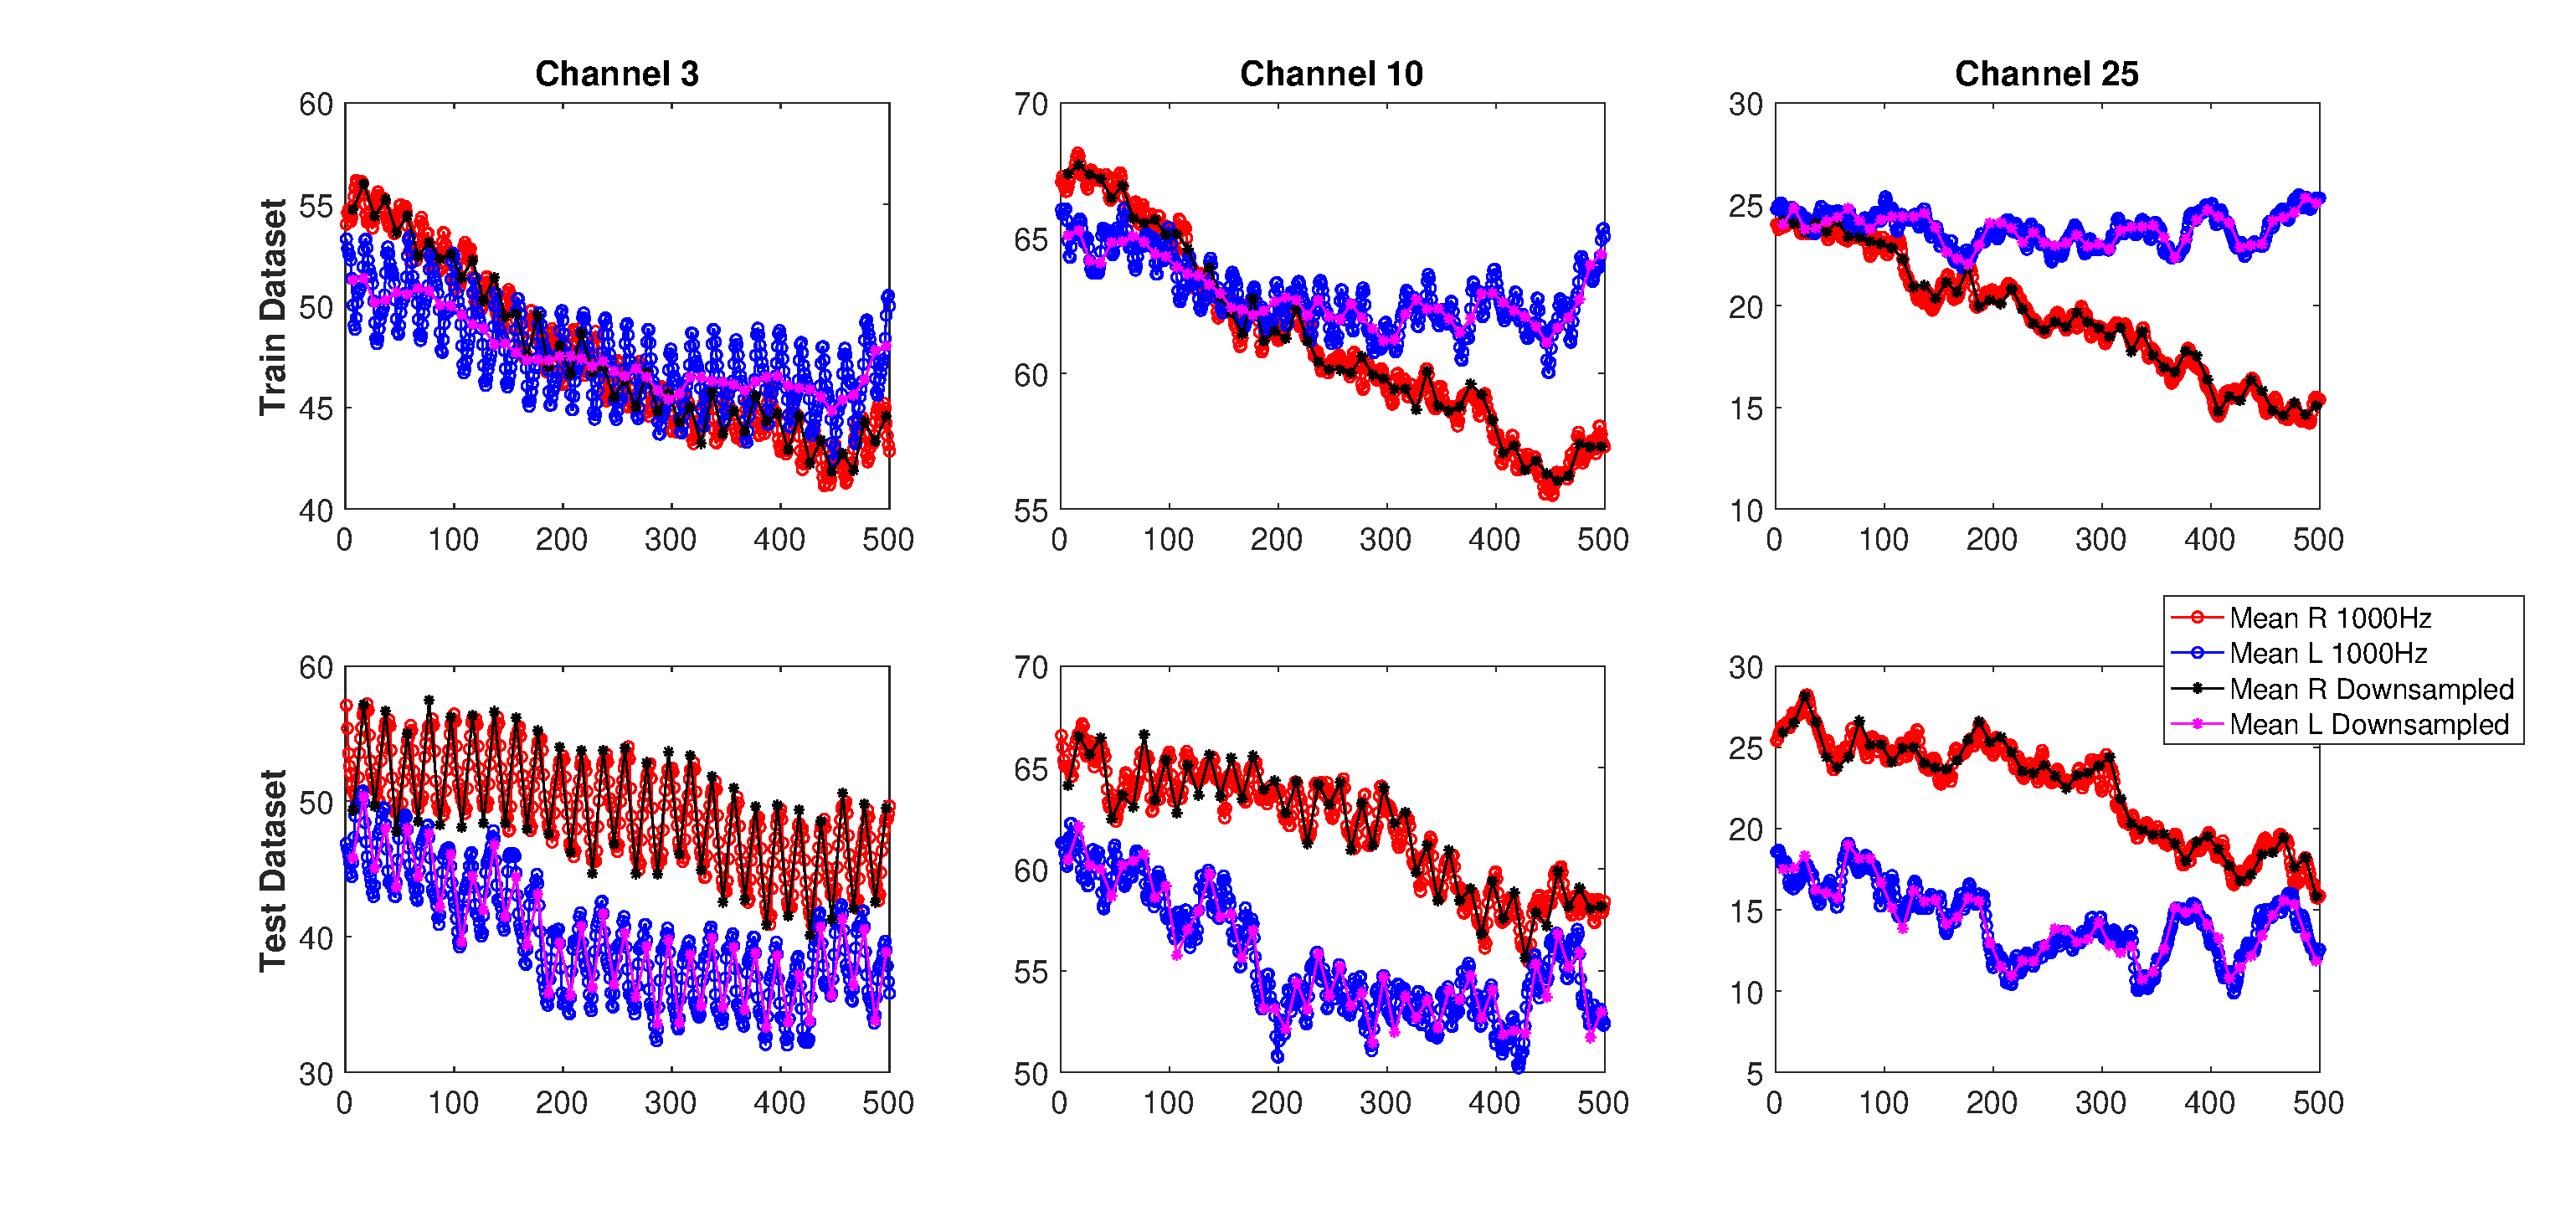
\includegraphics[width=1\textwidth]{fig/fig4new_mean_downsampled_vs1000} 
  \caption{Comparison of training and test datasets averages per channel over 316 and 100 samples, respectively.  
  Three channels (i.e., 3, 10 and 25) are randomly chosen, but the results generalise to all. 
  Each plot shows the mean of the samples with output 0 (i.e., classified as ``right'') and those with output 1 (i.e., classified as ``left''). 
  The means of the signals sampled with 1000 Hz are plotted in red and blue, while those of the signals downsampled to 100 Hz ar plotted in black and magenta. 
For some channels (e.g., channel 3) the down-sampled averages present a lower variability than those for the signals sampled at 1000 Hz. 
  In all cases, the averages of the training set are distinctively different from those of the test set. 
  \label{fig_mean_1000hz_vs_downsampled}}
  \end{center}
  \end{figure}t
  %
 This behaviour can be justified if  samples have a high variance and Figure \ref{fig_fewsamples_vs_mean_downsampled},which shows the behaviour of three randomly chosen down-sampled samples for each class (i.e., left and right) for both the training and test dataset, confirmes it. 
 Immediately, we can see that both the training and test selected samples are all very noisy and distant from their corresponding mean.
  \begin{figure}[h]
 \begin{center}
  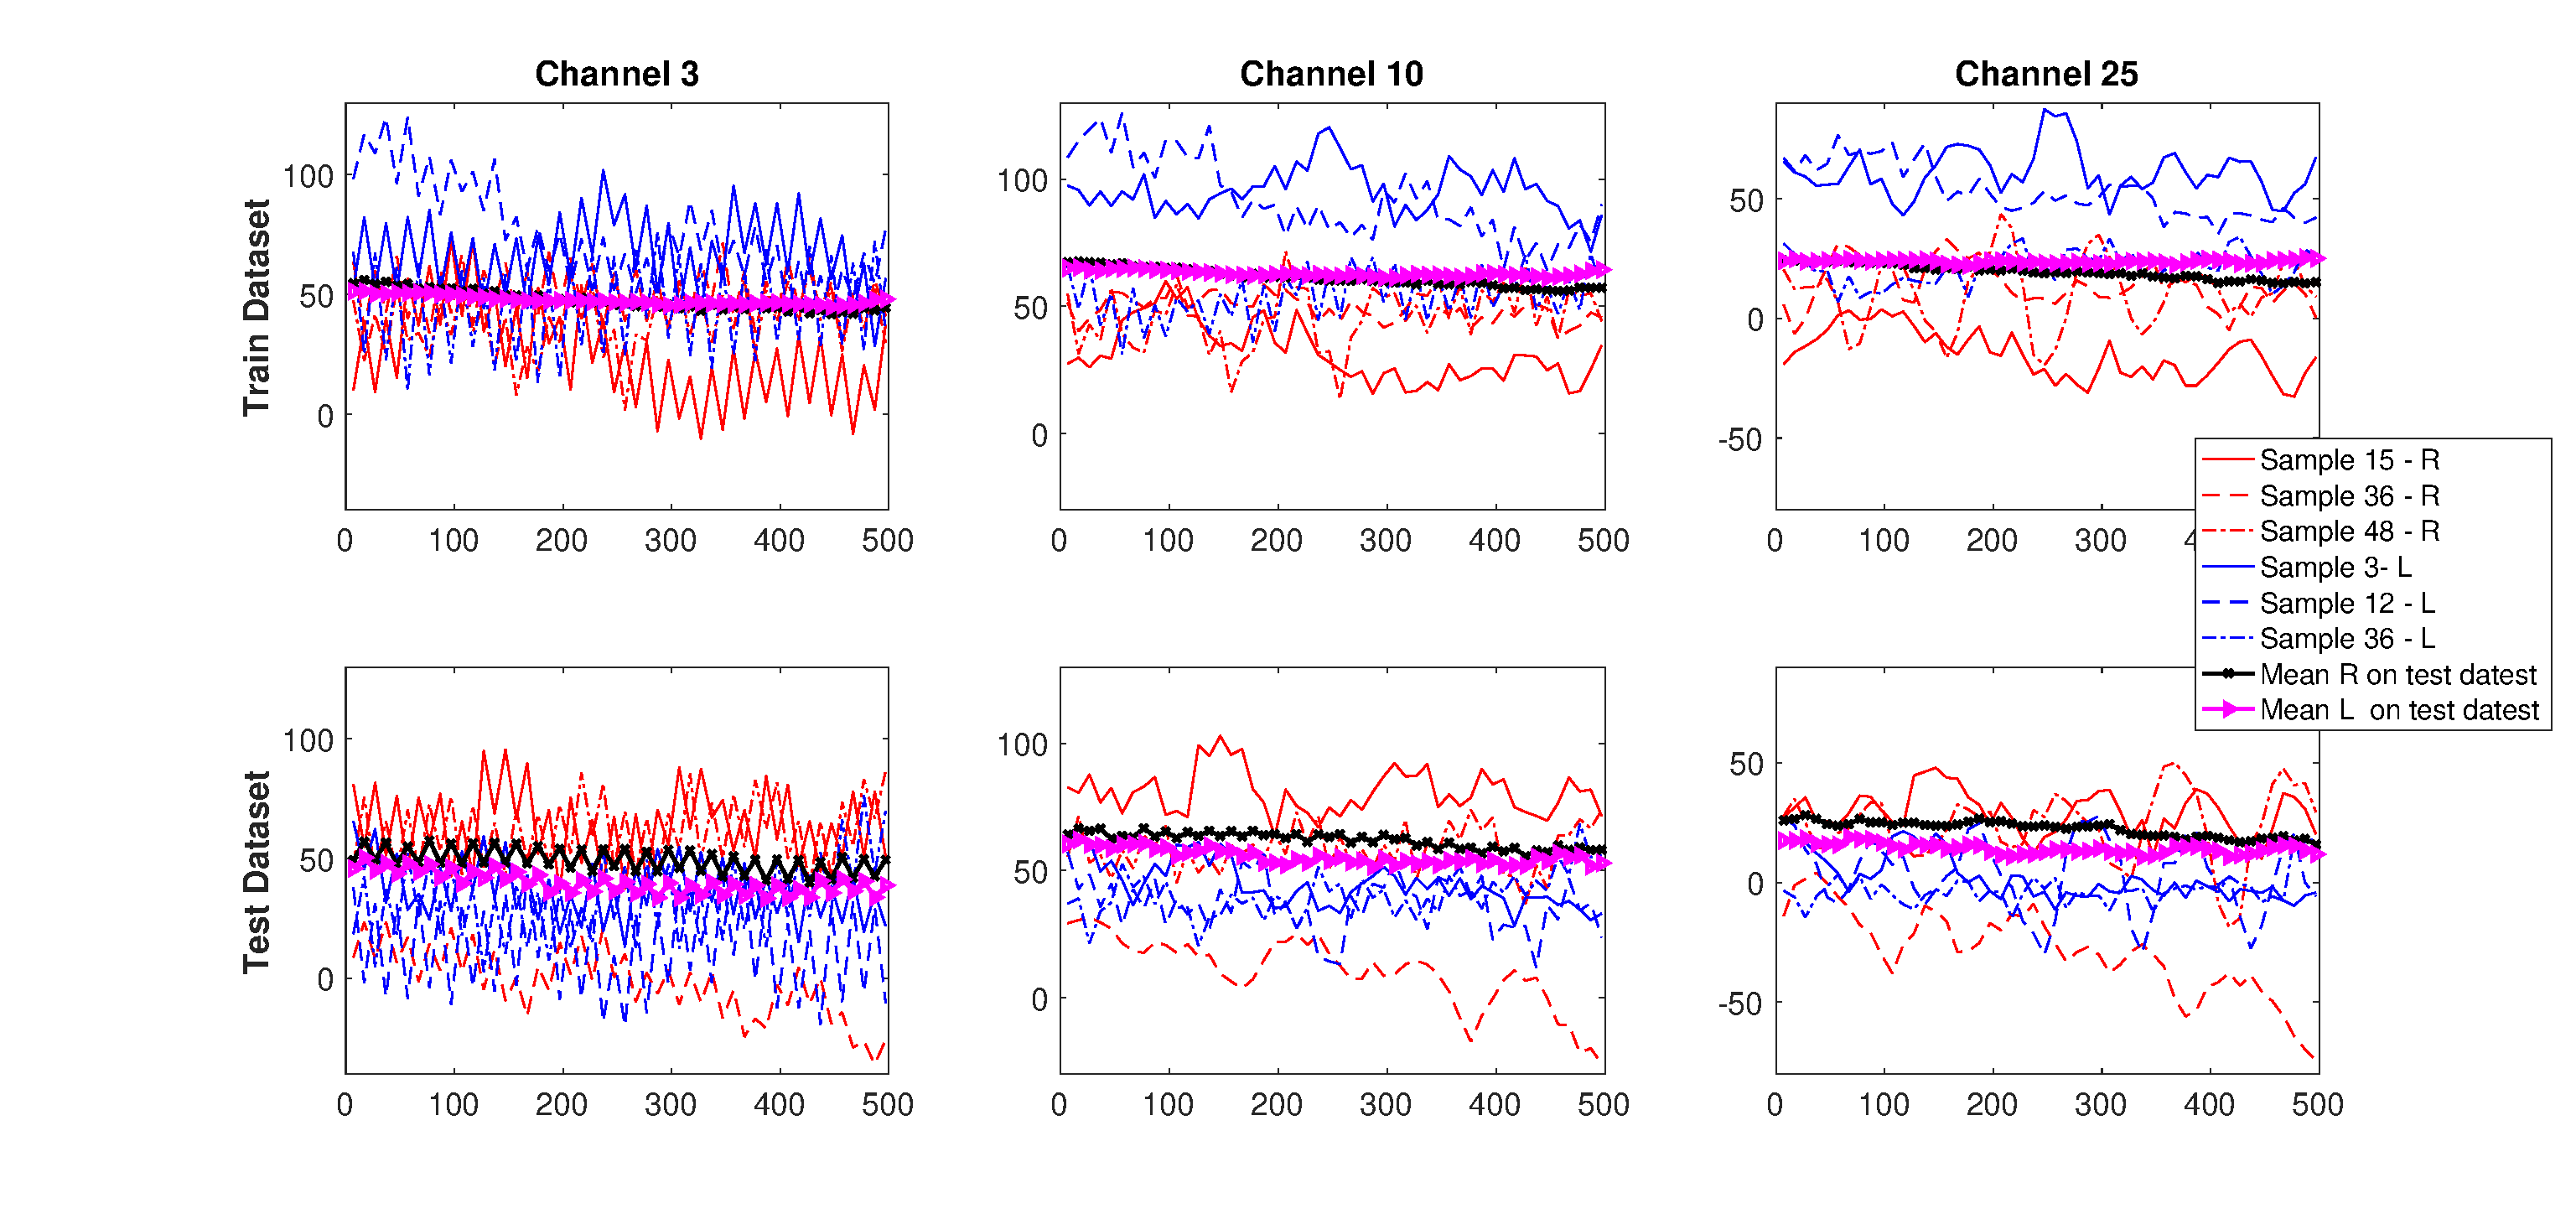
\includegraphics[width=1\textwidth]{fig/fig5new_fewsamples_mean_downsampled} 
  \caption{Plot of few randomly chosen samples from training and test datasets for channels 3, 10 and 25.
  Samples classified as 0 (i.e., ``right'') are plotted in red, while   samples classified as 1 (i.e., ``left'') are plotted in blue.
  The down-sampled averages corresponding to the training and test dataset are also shown in black.
   These plots confirm that the data have a high variability. 
  \label{fig_fewsamples_vs_mean_downsampled}}
  \end{center}
  \end{figure}
  
 Even if we understand that the average is not a sufficient meaningful quantity to describe a complex dataset, the high variability of data makes us believe that this apparently simple two-class 1D classification problem, will instead be quite challenging. 
  In order to reduce the discrepancies, we  normalise the training dataset using its mean and standard deviation for all channels. 
  The same values are used for the test dataset. 
  
Driven by the poor accuracy of the results obtained with the methods proposed in the next section, we decide to include a \emph{data-augmentation} strategy, which can be seen as a way of preprocesing the dataset and reduce the generalisation error \cite{goodfellow2016deep}. 
In particular, we exploit the 1000 Hz dataset to extract not one, but 10  signals with frequency 100 Hz. 
In this way, our training dataset has the following dimensions: 3160 samples, 28 channels, 50 time-steps. 
We considered the possibility of extending the data-augmentation strategy to the test dataset to further increase the dimension of our training dataset by including some samples from the test dataset after shuffling. 
However, we soon realised that this would imply solving an oversimplified problem being the 10 down-sampled signals all very alike. 
We therefore apply the data-augmentation strategy only to the training dataset. 


Finally, driven by the results already published for this dataset, known as dataset VI in the BCI competition \cite{bci_ii}, and supported by other studies (see e.g. \cite{schirrmeister2017deep}), we propose a preprocessing strategy to reduce both the generalisation error and the size of the model needed to fit the training set.
Indeed, by reducing the noise in the data, i.e., by increasing the signal-to-noise ration, we aim at reducing the amount of variation that the model has to take into account \cite{goodfellow2016deep} and thus . 
A \emph{filtering preprocessing} technique is therefore applied to our  final model, as explained in Section \ref{sec_themodel}.
In particular, we use the 1D Savitzky-Golay filter \cite{savgol} to smooth the data without greatly distorting the signal. 
By a convolution, the filter fits successive subsets of adjacent data points in a low-degree polynomial using the linear least squares method. 
In our tests, we use subsets of 7 points to be fitted in a polynomial of order 3.
Figure \ref{fig_smoothig_savgol} shows ....TODO
 \begin{figure}[h]
 \begin{center}
  \includegraphics[width=1\textwidth]{fig/fig6_smoothing} 
  \caption{lala
  \label{fig_smoothig_savgol}}
  \end{center}
  \end{figure}

 % TOADD ???  - mixed train+test mean? // train only 100 vs train 316 mean? 
 

 
 \section{Models we tried and why they don't work}\label{sec_allmodel}
 
 - Linear Perceptron --  Error train vs. test when overfitting 
 
 - Cross Validation (how many?)
 
 - Each model is averaged over N times 
 
 \begin{table}
 \begin{center}
    \begin{tabular}{|  c | c | c  | c |c |}
    \hline
    Number of trials & Linear & ConvNet1 & ConvNet2 & Shallow ConvNet \\ \hline
    1 & 29 & 34 & 37 & 29 \\
    2 & 27 & 29 & 34 & 27\\
    3 & 29 & 33 & 42 & 25\\
    4 & 37 & 36 & 28 & 29 \\
    5 & 31& 34 & 30 & 27 \\
    6 & & & & 29 \\
    7 & & & & 34\\
    8 & & & & 30 \\
    9 & & & & 36 \\
    10 & & & & 29 \\
        \hline
    Best & 27  & 29 & 28 &27 \\
    Average & & & &\\
    Variance & & & &\\
        \hline
    \end{tabular}
        \caption{Test errors}
\end{center}
\end{table}



 - 2 Conv 1D + 3 linear 
 
 - Conv only in the direction of the channels \cite{zheng2014time}
 
 - Conv with "images", i.e. Conv 2D asymmetric (only in one direction) \cite{schirrmeister2017deep}
 
 - All of them with Data Augmentation + white random noise \cite{wang2018data}
 
 -  adaptive eta in gradient descent 
 
 - L1 and L2 and other regularization techniques  \cite{goodfellow2016deep} 
 
 - dropout 
 
 -eta is reduced to 1e-3 when not converging
 
 
  \section{Model that works best}\label{sec_themodel}
 
 it doesnt overfit + graph
 
 
 -- Optimization with Hyperparameters
  
 \section{Conclusion}\label{sec_conclusion}
 
 
 % References
\bibliographystyle{abbrv}
\bibliography{mybib_dl} 
  
  
  
\end{document}